\documentclass[]{book}
\usepackage{lmodern}
\usepackage{amssymb,amsmath}
\usepackage{ifxetex,ifluatex}
\usepackage{fixltx2e} % provides \textsubscript
\ifnum 0\ifxetex 1\fi\ifluatex 1\fi=0 % if pdftex
  \usepackage[T1]{fontenc}
  \usepackage[utf8]{inputenc}
\else % if luatex or xelatex
  \ifxetex
    \usepackage{mathspec}
  \else
    \usepackage{fontspec}
  \fi
  \defaultfontfeatures{Ligatures=TeX,Scale=MatchLowercase}
\fi
% use upquote if available, for straight quotes in verbatim environments
\IfFileExists{upquote.sty}{\usepackage{upquote}}{}
% use microtype if available
\IfFileExists{microtype.sty}{%
\usepackage{microtype}
\UseMicrotypeSet[protrusion]{basicmath} % disable protrusion for tt fonts
}{}
\usepackage[margin=1in]{geometry}
\usepackage{hyperref}
\hypersetup{unicode=true,
            pdftitle={Data Science for Biological, Medical and Health Research: Notes for 432},
            pdfauthor={Thomas E. Love, Ph.D.},
            pdfborder={0 0 0},
            breaklinks=true}
\urlstyle{same}  % don't use monospace font for urls
\usepackage{natbib}
\bibliographystyle{apalike}
\usepackage{color}
\usepackage{fancyvrb}
\newcommand{\VerbBar}{|}
\newcommand{\VERB}{\Verb[commandchars=\\\{\}]}
\DefineVerbatimEnvironment{Highlighting}{Verbatim}{commandchars=\\\{\}}
% Add ',fontsize=\small' for more characters per line
\usepackage{framed}
\definecolor{shadecolor}{RGB}{248,248,248}
\newenvironment{Shaded}{\begin{snugshade}}{\end{snugshade}}
\newcommand{\KeywordTok}[1]{\textcolor[rgb]{0.13,0.29,0.53}{\textbf{#1}}}
\newcommand{\DataTypeTok}[1]{\textcolor[rgb]{0.13,0.29,0.53}{#1}}
\newcommand{\DecValTok}[1]{\textcolor[rgb]{0.00,0.00,0.81}{#1}}
\newcommand{\BaseNTok}[1]{\textcolor[rgb]{0.00,0.00,0.81}{#1}}
\newcommand{\FloatTok}[1]{\textcolor[rgb]{0.00,0.00,0.81}{#1}}
\newcommand{\ConstantTok}[1]{\textcolor[rgb]{0.00,0.00,0.00}{#1}}
\newcommand{\CharTok}[1]{\textcolor[rgb]{0.31,0.60,0.02}{#1}}
\newcommand{\SpecialCharTok}[1]{\textcolor[rgb]{0.00,0.00,0.00}{#1}}
\newcommand{\StringTok}[1]{\textcolor[rgb]{0.31,0.60,0.02}{#1}}
\newcommand{\VerbatimStringTok}[1]{\textcolor[rgb]{0.31,0.60,0.02}{#1}}
\newcommand{\SpecialStringTok}[1]{\textcolor[rgb]{0.31,0.60,0.02}{#1}}
\newcommand{\ImportTok}[1]{#1}
\newcommand{\CommentTok}[1]{\textcolor[rgb]{0.56,0.35,0.01}{\textit{#1}}}
\newcommand{\DocumentationTok}[1]{\textcolor[rgb]{0.56,0.35,0.01}{\textbf{\textit{#1}}}}
\newcommand{\AnnotationTok}[1]{\textcolor[rgb]{0.56,0.35,0.01}{\textbf{\textit{#1}}}}
\newcommand{\CommentVarTok}[1]{\textcolor[rgb]{0.56,0.35,0.01}{\textbf{\textit{#1}}}}
\newcommand{\OtherTok}[1]{\textcolor[rgb]{0.56,0.35,0.01}{#1}}
\newcommand{\FunctionTok}[1]{\textcolor[rgb]{0.00,0.00,0.00}{#1}}
\newcommand{\VariableTok}[1]{\textcolor[rgb]{0.00,0.00,0.00}{#1}}
\newcommand{\ControlFlowTok}[1]{\textcolor[rgb]{0.13,0.29,0.53}{\textbf{#1}}}
\newcommand{\OperatorTok}[1]{\textcolor[rgb]{0.81,0.36,0.00}{\textbf{#1}}}
\newcommand{\BuiltInTok}[1]{#1}
\newcommand{\ExtensionTok}[1]{#1}
\newcommand{\PreprocessorTok}[1]{\textcolor[rgb]{0.56,0.35,0.01}{\textit{#1}}}
\newcommand{\AttributeTok}[1]{\textcolor[rgb]{0.77,0.63,0.00}{#1}}
\newcommand{\RegionMarkerTok}[1]{#1}
\newcommand{\InformationTok}[1]{\textcolor[rgb]{0.56,0.35,0.01}{\textbf{\textit{#1}}}}
\newcommand{\WarningTok}[1]{\textcolor[rgb]{0.56,0.35,0.01}{\textbf{\textit{#1}}}}
\newcommand{\AlertTok}[1]{\textcolor[rgb]{0.94,0.16,0.16}{#1}}
\newcommand{\ErrorTok}[1]{\textcolor[rgb]{0.64,0.00,0.00}{\textbf{#1}}}
\newcommand{\NormalTok}[1]{#1}
\usepackage{longtable,booktabs}
\usepackage{graphicx,grffile}
\makeatletter
\def\maxwidth{\ifdim\Gin@nat@width>\linewidth\linewidth\else\Gin@nat@width\fi}
\def\maxheight{\ifdim\Gin@nat@height>\textheight\textheight\else\Gin@nat@height\fi}
\makeatother
% Scale images if necessary, so that they will not overflow the page
% margins by default, and it is still possible to overwrite the defaults
% using explicit options in \includegraphics[width, height, ...]{}
\setkeys{Gin}{width=\maxwidth,height=\maxheight,keepaspectratio}
\IfFileExists{parskip.sty}{%
\usepackage{parskip}
}{% else
\setlength{\parindent}{0pt}
\setlength{\parskip}{6pt plus 2pt minus 1pt}
}
\setlength{\emergencystretch}{3em}  % prevent overfull lines
\providecommand{\tightlist}{%
  \setlength{\itemsep}{0pt}\setlength{\parskip}{0pt}}
\setcounter{secnumdepth}{5}
% Redefines (sub)paragraphs to behave more like sections
\ifx\paragraph\undefined\else
\let\oldparagraph\paragraph
\renewcommand{\paragraph}[1]{\oldparagraph{#1}\mbox{}}
\fi
\ifx\subparagraph\undefined\else
\let\oldsubparagraph\subparagraph
\renewcommand{\subparagraph}[1]{\oldsubparagraph{#1}\mbox{}}
\fi

%%% Use protect on footnotes to avoid problems with footnotes in titles
\let\rmarkdownfootnote\footnote%
\def\footnote{\protect\rmarkdownfootnote}

%%% Change title format to be more compact
\usepackage{titling}

% Create subtitle command for use in maketitle
\newcommand{\subtitle}[1]{
  \posttitle{
    \begin{center}\large#1\end{center}
    }
}

\setlength{\droptitle}{-2em}
  \title{Data Science for Biological, Medical and Health Research: Notes for 432}
  \pretitle{\vspace{\droptitle}\centering\huge}
  \posttitle{\par}
  \author{Thomas E. Love, Ph.D.}
  \preauthor{\centering\large\emph}
  \postauthor{\par}
  \predate{\centering\large\emph}
  \postdate{\par}
  \date{Version: 2018-01-15}

\usepackage{booktabs}
\usepackage{amsthm}
\makeatletter
\def\thm@space@setup{%
  \thm@preskip=8pt plus 2pt minus 4pt
  \thm@postskip=\thm@preskip
}
\makeatother

\usepackage{amsthm}
\newtheorem{theorem}{Theorem}[chapter]
\newtheorem{lemma}{Lemma}[chapter]
\theoremstyle{definition}
\newtheorem{definition}{Definition}[chapter]
\newtheorem{corollary}{Corollary}[chapter]
\newtheorem{proposition}{Proposition}[chapter]
\theoremstyle{definition}
\newtheorem{example}{Example}[chapter]
\theoremstyle{definition}
\newtheorem{exercise}{Exercise}[chapter]
\theoremstyle{remark}
\newtheorem*{remark}{Remark}
\newtheorem*{solution}{Solution}
\begin{document}
\maketitle

{
\setcounter{tocdepth}{1}
\tableofcontents
}
\chapter*{Introduction}\label{introduction}
\addcontentsline{toc}{chapter}{Introduction}

These Notes provide a series of examples using R to work through issues
that are likely to come up in PQHS/CRSP/MPHP 432.

While these Notes share some of the features of a textbook, they are
neither comprehensive nor completely original. The main purpose is to
give students in 432 a set of common materials on which to draw during
the course. In class, we will sometimes:

\begin{itemize}
\tightlist
\item
  reiterate points made in this document,
\item
  amplify what is here,
\item
  simplify the presentation of things done here,
\item
  use new examples to show some of the same techniques,
\item
  refer to issues not mentioned in this document,
\end{itemize}

but what we don't (always) do is follow these notes very precisely. We
assume instead that you will read the materials and try to learn from
them, just as you will attend classes and try to learn from them. We
welcome feedback of all kinds on this document or anything else. Just
email us at \texttt{431-help\ at\ case\ dot\ edu}, or submit a pull
request. Note that we still use \texttt{431-help} even though we're now
in 432.

What you will mostly find are brief explanations of a key idea or
summary, accompanied (most of the time) by R code and a demonstration of
the results of applying that code.

Everything you see here is available to you as HTML or PDF. You will
also have access to the R Markdown files, which contain the code which
generates everything in the document, including all of the R results. We
will demonstrate the use of R Markdown (this document is generated with
the additional help of an R package called bookdown) and R Studio (the
``program'' which we use to interface with the R language) in class.

To download the data and R code related to these notes, visit the Data
and Code section of \href{https://github.com/THOMASELOVE/432-2018}{the
432 course website}.

\chapter*{R Packages used in these
notes}\label{r-packages-used-in-these-notes}
\addcontentsline{toc}{chapter}{R Packages used in these notes}

Here, we'll load in the packages used in these notes.

\begin{Shaded}
\begin{Highlighting}[]
\KeywordTok{library}\NormalTok{(tableone)}
\KeywordTok{library}\NormalTok{(skimr)}
\KeywordTok{library}\NormalTok{(broom)}
\KeywordTok{library}\NormalTok{(tidyverse)}
\end{Highlighting}
\end{Shaded}

\chapter*{Data used in these notes}\label{data-used-in-these-notes}
\addcontentsline{toc}{chapter}{Data used in these notes}

Here, we'll load in the data sets used in these notes.

\begin{Shaded}
\begin{Highlighting}[]
\NormalTok{fakestroke <-}\StringTok{ }\KeywordTok{read.csv}\NormalTok{(}\StringTok{"data/fakestroke.csv"}\NormalTok{) }\OperatorTok\StringTok{ }\NormalTok{tbl_df}
\NormalTok{bloodbrain <-}\StringTok{ }\KeywordTok{read.csv}\NormalTok{(}\StringTok{"data/bloodbrain.csv"}\NormalTok{) }\OperatorTok\StringTok{ }\NormalTok{tbl_df}
\NormalTok{smartcle1 <-}\StringTok{ }\KeywordTok{read.csv}\NormalTok{(}\StringTok{"data/smartcle1.csv"}\NormalTok{) }\OperatorTok\StringTok{ }\NormalTok{tbl_df}
\end{Highlighting}
\end{Shaded}

\chapter{Building Table 1}\label{building-table-1}

Many scientific articles involve direct comparison of results from
various exposures, perhaps treatments. In 431, we studied numerous
methods, including various sorts of hypothesis tests, confidence
intervals, and descriptive summaries, which can help us to understand
and compare outcomes in such a setting. One common approach is to
present what's often called Table 1. Table 1 provides a summary of the
characteristics of a sample, or of groups of samples, which is most
commonly used to help understand the nature of the data being compared.

\section{\texorpdfstring{Two examples from the \emph{New England Journal
of
Medicine}}{Two examples from the New England Journal of Medicine}}\label{two-examples-from-the-new-england-journal-of-medicine}

\subsection{A simple Table 1}\label{a-simple-table-1}

Table 1 is especially common in the context of clinical research.
Consider the excerpt below, from a January 2015 article in the \emph{New
England Journal of Medicine} \citep{Tolaney2015}.

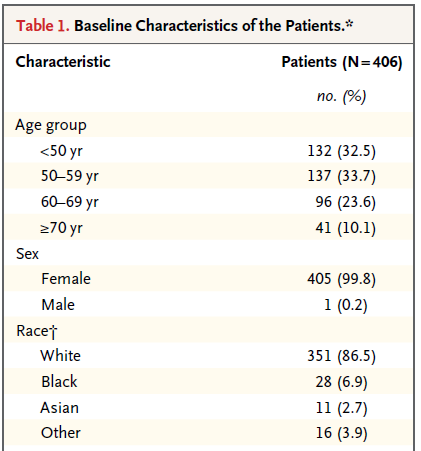
\includegraphics[width=0.5\linewidth]{images/Tolaney-snip1}

This (partial) table reports baseline characteristics on age group, sex
and race, describing 406 patients with HER2-positive\footnote{HER2 =
  human epidermal growth factor receptor type 2. Over-expression of this
  occurs in 15-20\% of invasive breast cancers, and has been associated
  with poor outcomes.} invasive breast cancer that began the protocol
therapy. Age, sex and race (along with severity of illness) are the most
commonly identified characteristics in a Table 1.

In addition to the measures shown in this excerpt, the full Table also
includes detailed information on the primary tumor for each patient,
including its size, nodal status and histologic grade. Footnotes tell us
that the percentages shown are subject to rounding, and may not total
100, and that the race information was self-reported.

\subsection{A group comparison}\label{a-group-comparison}

A more typical Table 1 involves a group comparison, for example in this
excerpt from \citet{Roy2008}. This Table 1 describes a multi-center
randomized clinical trial comparing two different approaches to caring
for patients with heart failure and atrial fibrillation\footnote{The
  complete Table 1 appears on pages 2668-2669 of \citet{Roy2008}, but I
  have only reproduced the first page and the footnote in this excerpt.}.

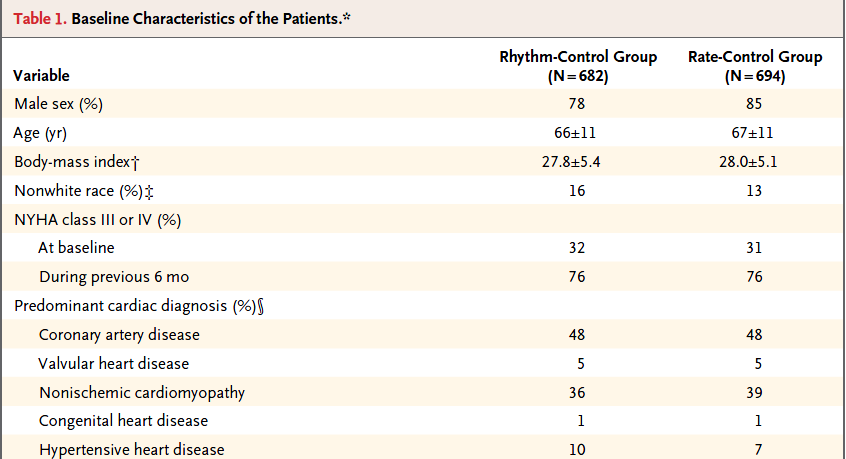
\includegraphics[width=0.9\linewidth]{images/Roy-snip1}

The article provides percentages, means and standard deviations across
groups, but note that it does not provide p values for the comparison of
baseline characteristics. This is a common feature of NEJM reports on
randomized clinical trials, where we anticipate that the two groups will
be well matched at baseline. Note that the patients in this study were
\emph{randomly} assigned to either the rhythm-control group or to the
rate-control group, using blocked randomizations stratified by study
center.

\section{The MR CLEAN trial}\label{the-mr-clean-trial}

\citet{Berkhemer2015} reported on the MR CLEAN trial, involving 500
patients with acute ischemic stroke caused by a proximal intracranial
arterial occlusion. The trial was conducted at 16 medical centers in the
Netherlands, where 233 were randomly assigned to the intervention
(intraarterial treatment plus usual care) and 267 to control (usual care
alone.) The primary outcome was the modified Rankin scale score at 90
days; this categorical scale measures functional outcome, with scores
ranging from 0 (no symptoms) to 6 (death). The fundamental conclusion of
\citet{Berkhemer2015} was that in patients with acute ischemic stroke
caused by a proximal intracranial occlusion of the anterior circulation,
intraarterial treatment administered within 6 hours after stroke onset
was effective and safe.

Here's the Table 1 from \citet{Berkhemer2015}.

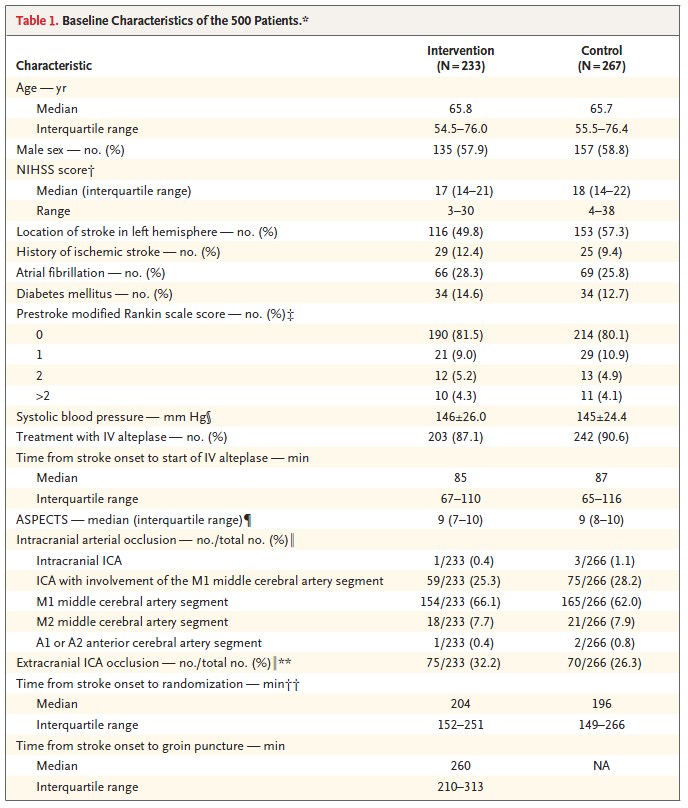
\includegraphics[width=0.9\linewidth]{images/Berkhemer-snip4complete}

The Table was accompanied by the following notes.

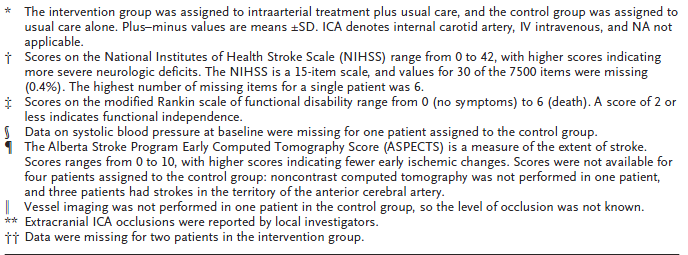
\includegraphics[width=0.9\linewidth]{images/Berkhemer-snip4notes}

\section{\texorpdfstring{Simulated \texttt{fakestroke}
data}{Simulated fakestroke data}}\label{simulated-fakestroke-data}

Consider the simulated data, available on the Data and Code page of
\href{https://github.com/THOMASELOVE/432-2018}{our course website} in
the \texttt{fakestroke.csv} file, which I built to let us mirror the
Table 1 for MR CLEAN \citep{Berkhemer2015}. The \texttt{fakestroke.csv}
file contains the following 18 variables for 500 patients.

\begin{longtable}[]{@{}rl@{}}
\toprule
\begin{minipage}[b]{0.16\columnwidth}\raggedleft\strut
Variable\strut
\end{minipage} & \begin{minipage}[b]{0.55\columnwidth}\raggedright\strut
Description\strut
\end{minipage}\tabularnewline
\midrule
\endhead
\begin{minipage}[t]{0.16\columnwidth}\raggedleft\strut
\texttt{studyid}\strut
\end{minipage} & \begin{minipage}[t]{0.55\columnwidth}\raggedright\strut
Study ID \# (z001 through z500)\strut
\end{minipage}\tabularnewline
\begin{minipage}[t]{0.16\columnwidth}\raggedleft\strut
\texttt{trt}\strut
\end{minipage} & \begin{minipage}[t]{0.55\columnwidth}\raggedright\strut
Treatment group (Intervention or Control)\strut
\end{minipage}\tabularnewline
\begin{minipage}[t]{0.16\columnwidth}\raggedleft\strut
\texttt{age}\strut
\end{minipage} & \begin{minipage}[t]{0.55\columnwidth}\raggedright\strut
Age in years\strut
\end{minipage}\tabularnewline
\begin{minipage}[t]{0.16\columnwidth}\raggedleft\strut
\texttt{sex}\strut
\end{minipage} & \begin{minipage}[t]{0.55\columnwidth}\raggedright\strut
Male or Female\strut
\end{minipage}\tabularnewline
\begin{minipage}[t]{0.16\columnwidth}\raggedleft\strut
\texttt{nihss}\strut
\end{minipage} & \begin{minipage}[t]{0.55\columnwidth}\raggedright\strut
NIH Stroke Scale Score (can range from 0-42; higher scores indicate more
severe neurological deficits)\strut
\end{minipage}\tabularnewline
\begin{minipage}[t]{0.16\columnwidth}\raggedleft\strut
\texttt{location}\strut
\end{minipage} & \begin{minipage}[t]{0.55\columnwidth}\raggedright\strut
Stroke Location - Left or Right Hemisphere\strut
\end{minipage}\tabularnewline
\begin{minipage}[t]{0.16\columnwidth}\raggedleft\strut
\texttt{hx.isch}\strut
\end{minipage} & \begin{minipage}[t]{0.55\columnwidth}\raggedright\strut
History of Ischemic Stroke (Yes/No)\strut
\end{minipage}\tabularnewline
\begin{minipage}[t]{0.16\columnwidth}\raggedleft\strut
\texttt{afib}\strut
\end{minipage} & \begin{minipage}[t]{0.55\columnwidth}\raggedright\strut
Atrial Fibrillation (1 = Yes, 0 = No)\strut
\end{minipage}\tabularnewline
\begin{minipage}[t]{0.16\columnwidth}\raggedleft\strut
\texttt{dm}\strut
\end{minipage} & \begin{minipage}[t]{0.55\columnwidth}\raggedright\strut
Diabetes Mellitus (1 = Yes, 0 = No)\strut
\end{minipage}\tabularnewline
\begin{minipage}[t]{0.16\columnwidth}\raggedleft\strut
\texttt{mrankin}\strut
\end{minipage} & \begin{minipage}[t]{0.55\columnwidth}\raggedright\strut
Pre-stroke modified Rankin scale score (0, 1, 2 or \textgreater{} 2)
indicating functional disability - complete range is 0 (no symptoms) to
6 (death)\strut
\end{minipage}\tabularnewline
\begin{minipage}[t]{0.16\columnwidth}\raggedleft\strut
\texttt{sbp}\strut
\end{minipage} & \begin{minipage}[t]{0.55\columnwidth}\raggedright\strut
Systolic blood pressure, in mm Hg\strut
\end{minipage}\tabularnewline
\begin{minipage}[t]{0.16\columnwidth}\raggedleft\strut
\texttt{iv.altep}\strut
\end{minipage} & \begin{minipage}[t]{0.55\columnwidth}\raggedright\strut
Treatment with IV alteplase (Yes/No)\strut
\end{minipage}\tabularnewline
\begin{minipage}[t]{0.16\columnwidth}\raggedleft\strut
\texttt{time.iv}\strut
\end{minipage} & \begin{minipage}[t]{0.55\columnwidth}\raggedright\strut
Time from stroke onset to start of IV alteplase (minutes) if
iv.altep=Yes\strut
\end{minipage}\tabularnewline
\begin{minipage}[t]{0.16\columnwidth}\raggedleft\strut
\texttt{aspects}\strut
\end{minipage} & \begin{minipage}[t]{0.55\columnwidth}\raggedright\strut
Alberta Stroke Program Early Computed Tomography score, which measures
extent of stroke from 0 - 10; higher scores indicate fewer early
ischemic changes\strut
\end{minipage}\tabularnewline
\begin{minipage}[t]{0.16\columnwidth}\raggedleft\strut
\texttt{ia.occlus}\strut
\end{minipage} & \begin{minipage}[t]{0.55\columnwidth}\raggedright\strut
Intracranial arterial occlusion, based on vessel imaging - five
categories\footnotemark{}\strut
\end{minipage}
\footnotetext{The five categories are Intracranial ICA, ICA with
  involvement of the M1 middle cerebral artery segment, M1 middle
  cerebral artery segment, M2 middle cerebral artery segment, A1 or A2
  anterior cerebral artery segment}\tabularnewline
\begin{minipage}[t]{0.16\columnwidth}\raggedleft\strut
\texttt{extra.ica}\strut
\end{minipage} & \begin{minipage}[t]{0.55\columnwidth}\raggedright\strut
Extracranial ICA occlusion (1 = Yes, 0 = No)\strut
\end{minipage}\tabularnewline
\begin{minipage}[t]{0.16\columnwidth}\raggedleft\strut
\texttt{time.rand}\strut
\end{minipage} & \begin{minipage}[t]{0.55\columnwidth}\raggedright\strut
Time from stroke onset to study randomization, in minutes\strut
\end{minipage}\tabularnewline
\begin{minipage}[t]{0.16\columnwidth}\raggedleft\strut
\texttt{time.punc}\strut
\end{minipage} & \begin{minipage}[t]{0.55\columnwidth}\raggedright\strut
Time from stroke onset to groin puncture, in minutes (only if
Intervention)\strut
\end{minipage}\tabularnewline
\bottomrule
\end{longtable}

Here's a quick look at the simulated data in \texttt{fakestroke}.

\begin{Shaded}
\begin{Highlighting}[]
\NormalTok{fakestroke}
\end{Highlighting}
\end{Shaded}

\begin{verbatim}
# A tibble: 500 x 18
   studyid trt        age sex   nihss location hx.isch  afib    dm mrankin
   <fct>   <fct>    <dbl> <fct> <int> <fct>    <fct>   <int> <int> <fct>  
 1 z001    Control   53.0 Male     21 Right    No          0     0 2      
 2 z002    Interve~  51.0 Male     23 Left     No          1     0 0      
 3 z003    Control   68.0 Fema~    11 Right    No          0     0 0      
 4 z004    Control   28.0 Male     22 Left     No          0     0 0      
 5 z005    Control   91.0 Male     24 Right    No          0     0 0      
 6 z006    Control   34.0 Fema~    18 Left     No          0     0 2      
 7 z007    Interve~  75.0 Male     25 Right    No          0     0 0      
 8 z008    Control   89.0 Fema~    18 Right    No          0     0 0      
 9 z009    Control   75.0 Male     25 Left     No          1     0 2      
10 z010    Interve~  26.0 Fema~    27 Right    No          0     0 0      
# ... with 490 more rows, and 8 more variables: sbp <int>, iv.altep <fct>,
#   time.iv <int>, aspects <int>, ia.occlus <fct>, extra.ica <int>,
#   time.rand <int>, time.punc <int>
\end{verbatim}

\section{\texorpdfstring{Building Table 1 for \texttt{fakestroke}:
Attempt
1}{Building Table 1 for fakestroke: Attempt 1}}\label{building-table-1-for-fakestroke-attempt-1}

Our goal, then, is to take the data in \texttt{fakestroke.csv} and use
it to generate a Table 1 for the study that compares the 233 patients in
the Intervention group to the 267 patients in the Control group, on all
of the other variables (except study ID \#) available. I'll use the
\texttt{tableone} package of functions available in R to help me
complete this task. We'll make a first attempt, using the
\texttt{CreateTableOne} function in the \texttt{tableone} package. To
use the function, we'll need to specify:

\begin{itemize}
\tightlist
\item
  the \texttt{vars} or variables we want to place in the rows of our
  Table 1 (which will include just about everything in the
  \texttt{fakestroke} data except the \texttt{studyid} code and the
  \texttt{trt} variable for which we have other plans, and the
  \texttt{time.punc} which applies only to subjects in the Intervention
  group.)

  \begin{itemize}
  \tightlist
  \item
    A useful trick here is to use the \texttt{dput} function,
    specifically something like \texttt{dput(names(fakestroke))} can be
    used to generate a list of all of the variables included in the
    \texttt{fakestroke} tibble, and then this can be copied and pasted
    into the \texttt{vars} specification, saving some typing.
  \end{itemize}
\item
  the \texttt{strata} which indicates the levels want to use in the
  columns of our Table 1 (for us, that's \texttt{trt})
\end{itemize}

\begin{Shaded}
\begin{Highlighting}[]
\NormalTok{fs.vars <-}\StringTok{ }\KeywordTok{c}\NormalTok{(}\StringTok{"age"}\NormalTok{, }\StringTok{"sex"}\NormalTok{, }\StringTok{"nihss"}\NormalTok{, }\StringTok{"location"}\NormalTok{, }
          \StringTok{"hx.isch"}\NormalTok{, }\StringTok{"afib"}\NormalTok{, }\StringTok{"dm"}\NormalTok{, }\StringTok{"mrankin"}\NormalTok{, }\StringTok{"sbp"}\NormalTok{,}
          \StringTok{"iv.altep"}\NormalTok{, }\StringTok{"time.iv"}\NormalTok{, }\StringTok{"aspects"}\NormalTok{, }
          \StringTok{"ia.occlus"}\NormalTok{, }\StringTok{"extra.ica"}\NormalTok{, }\StringTok{"time.rand"}\NormalTok{)}

\NormalTok{fs.trt <-}\StringTok{ }\KeywordTok{c}\NormalTok{(}\StringTok{"trt"}\NormalTok{)}

\NormalTok{att1 <-}\StringTok{ }\KeywordTok{CreateTableOne}\NormalTok{(}\DataTypeTok{data =}\NormalTok{ fakestroke, }
                       \DataTypeTok{vars =}\NormalTok{ fs.vars, }
                       \DataTypeTok{strata =}\NormalTok{ fs.trt)}
\KeywordTok{print}\NormalTok{(att1)}
\end{Highlighting}
\end{Shaded}

\begin{verbatim}
                       Stratified by trt
                        Control        Intervention   p      test
  n                        267            233                    
  age (mean (sd))        65.38 (16.10)  63.93 (18.09)  0.343     
  sex = Male (%)           157 (58.8)     135 (57.9)   0.917     
  nihss (mean (sd))      18.08 (4.32)   17.97 (5.04)   0.787     
  location = Right (%)     114 (42.7)     117 (50.2)   0.111     
  hx.isch = Yes (%)         25 ( 9.4)      29 (12.4)   0.335     
  afib (mean (sd))        0.26 (0.44)    0.28 (0.45)   0.534     
  dm (mean (sd))          0.13 (0.33)    0.12 (0.33)   0.923     
  mrankin (%)                                          0.922     
     > 2                    11 ( 4.1)      10 ( 4.3)             
     0                     214 (80.1)     190 (81.5)             
     1                      29 (10.9)      21 ( 9.0)             
     2                      13 ( 4.9)      12 ( 5.2)             
  sbp (mean (sd))       145.00 (24.40) 146.03 (26.00)  0.647     
  iv.altep = Yes (%)       242 (90.6)     203 (87.1)   0.267     
  time.iv (mean (sd))    87.96 (26.01)  98.22 (45.48)  0.003     
  aspects (mean (sd))     8.65 (1.47)    8.35 (1.64)   0.033     
  ia.occlus (%)                                        0.795     
     A1 or A2                2 ( 0.8)       1 ( 0.4)             
     ICA with M1            75 (28.2)      59 (25.3)             
     Intracranial ICA        3 ( 1.1)       1 ( 0.4)             
     M1                    165 (62.0)     154 (66.1)             
     M2                     21 ( 7.9)      18 ( 7.7)             
  extra.ica (mean (sd))   0.26 (0.44)    0.32 (0.47)   0.150     
  time.rand (mean (sd)) 213.88 (70.29) 202.51 (57.33)  0.051     
\end{verbatim}

\subsection{Some of this is very useful, and other parts need to be
fixed.}\label{some-of-this-is-very-useful-and-other-parts-need-to-be-fixed.}

\begin{enumerate}
\def\labelenumi{\arabic{enumi}.}
\tightlist
\item
  The 1/0 variables (\texttt{afib}, \texttt{dm}, \texttt{extra.ica})
  might be better if they were treated as the factors they are, and
  reported as the Yes/No variables are reported, with counts and
  percentages rather than with means and standard deviations.
\item
  In some cases, we may prefer to re-order the levels of the categorical
  (factor) variables, particularly the \texttt{mrankin} variable, but
  also the \texttt{ia.occlus} variable. It would also be more typical to
  put the Intervention group to the left and the Control group to the
  right, so we may need to adjust our \texttt{trt} variable's levels
  accordingly.
\item
  For each of the quantitative variables (\texttt{age}, \texttt{nihss},
  \texttt{sbp}, \texttt{time.iv}, \texttt{aspects}, \texttt{extra.ica},
  \texttt{time.rand} and \texttt{time.punc}) we should make a decision
  whether a summary with mean and standard deviation is appropriate, or
  whether we should instead summarize with, say, the median and
  quartiles. A mean and standard deviation really only yields an
  appropriate summary when the data are least approximately Normally
  distributed. This will make the \emph{p} values a bit more reasonable,
  too. The \texttt{test} column in the first attempt will soon have
  something useful to tell us.
\item
  If we'd left in the \texttt{time.punc} variable, we'd get some
  warnings, having to do with the fact that \texttt{time.punc} is only
  relevant to patients in the Intervention group.
\end{enumerate}

\subsection{\texorpdfstring{\texttt{fakestroke} Cleaning Up Categorical
Variables}{fakestroke Cleaning Up Categorical Variables}}\label{fakestroke-cleaning-up-categorical-variables}

Let's specify each of the categorical variables as categorical
explicitly. This helps the \texttt{CreateTableOne} function treat them
appropriately, and display them with counts and percentages. This
includes all of the 1/0, Yes/No and multi-categorical variables.

\begin{Shaded}
\begin{Highlighting}[]
\NormalTok{fs.factorvars <-}\StringTok{ }\KeywordTok{c}\NormalTok{(}\StringTok{"sex"}\NormalTok{, }\StringTok{"location"}\NormalTok{, }\StringTok{"hx.isch"}\NormalTok{, }\StringTok{"afib"}\NormalTok{, }\StringTok{"dm"}\NormalTok{, }
                   \StringTok{"mrankin"}\NormalTok{, }\StringTok{"iv.altep"}\NormalTok{, }\StringTok{"ia.occlus"}\NormalTok{, }\StringTok{"extra.ica"}\NormalTok{)}
\end{Highlighting}
\end{Shaded}

Then we simply add a \texttt{factorVars\ =\ fs.factorvars} call to the
\texttt{CreateTableOne} function.

We also want to re-order some of those categorical variables, so that
the levels are more useful to us. Specifically, we want to:

\begin{itemize}
\tightlist
\item
  place Intervention before Control in the \texttt{trt} variable,
\item
  reorder the \texttt{mrankin} scale as 0, 1, 2, \textgreater{} 2, and
\item
  rearrange the \texttt{ia.occlus} variable to the order\footnote{We
    might also have considered reordering the \texttt{ia.occlus} factor
    by its frequency, using the \texttt{fct\_infreq} function} presented
  in \citet{Berkhemer2015}.
\end{itemize}

To accomplish this, we'll use the \texttt{fct\_relevel} function from
the \texttt{forcats} package (loaded with the rest of the core
\texttt{tidyverse} packages) to reorder our levels manually.

\begin{Shaded}
\begin{Highlighting}[]
\NormalTok{fakestroke <-}\StringTok{ }\NormalTok{fakestroke }\OperatorTok
\StringTok{    }\KeywordTok{mutate}\NormalTok{(}\DataTypeTok{trt =} \KeywordTok{fct_relevel}\NormalTok{(trt, }\StringTok{"Intervention"}\NormalTok{, }\StringTok{"Control"}\NormalTok{),}
           \DataTypeTok{mrankin =} \KeywordTok{fct_relevel}\NormalTok{(mrankin, }\StringTok{"0"}\NormalTok{, }\StringTok{"1"}\NormalTok{, }\StringTok{"2"}\NormalTok{, }\StringTok{"> 2"}\NormalTok{),}
           \DataTypeTok{ia.occlus =} \KeywordTok{fct_relevel}\NormalTok{(ia.occlus, }\StringTok{"Intracranial ICA"}\NormalTok{, }
                                   \StringTok{"ICA with M1"}\NormalTok{, }\StringTok{"M1"}\NormalTok{, }\StringTok{"M2"}\NormalTok{, }
                                   \StringTok{"A1 or A2"}\NormalTok{)}
\NormalTok{           ) }
\end{Highlighting}
\end{Shaded}

\section{\texorpdfstring{\texttt{fakestroke} Table 1: Attempt
2}{fakestroke Table 1: Attempt 2}}\label{fakestroke-table-1-attempt-2}

\begin{Shaded}
\begin{Highlighting}[]
\NormalTok{att2 <-}\StringTok{ }\KeywordTok{CreateTableOne}\NormalTok{(}\DataTypeTok{data =}\NormalTok{ fakestroke, }
                       \DataTypeTok{vars =}\NormalTok{ fs.vars,}
                       \DataTypeTok{factorVars =}\NormalTok{ fs.factorvars,}
                       \DataTypeTok{strata =}\NormalTok{ fs.trt)}
\KeywordTok{print}\NormalTok{(att2)}
\end{Highlighting}
\end{Shaded}

\begin{verbatim}
                       Stratified by trt
                        Intervention   Control        p      test
  n                        233            267                    
  age (mean (sd))        63.93 (18.09)  65.38 (16.10)  0.343     
  sex = Male (%)           135 (57.9)     157 (58.8)   0.917     
  nihss (mean (sd))      17.97 (5.04)   18.08 (4.32)   0.787     
  location = Right (%)     117 (50.2)     114 (42.7)   0.111     
  hx.isch = Yes (%)         29 (12.4)      25 ( 9.4)   0.335     
  afib = 1 (%)              66 (28.3)      69 (25.8)   0.601     
  dm = 1 (%)                29 (12.4)      34 (12.7)   1.000     
  mrankin (%)                                          0.922     
     0                     190 (81.5)     214 (80.1)             
     1                      21 ( 9.0)      29 (10.9)             
     2                      12 ( 5.2)      13 ( 4.9)             
     > 2                    10 ( 4.3)      11 ( 4.1)             
  sbp (mean (sd))       146.03 (26.00) 145.00 (24.40)  0.647     
  iv.altep = Yes (%)       203 (87.1)     242 (90.6)   0.267     
  time.iv (mean (sd))    98.22 (45.48)  87.96 (26.01)  0.003     
  aspects (mean (sd))     8.35 (1.64)    8.65 (1.47)   0.033     
  ia.occlus (%)                                        0.795     
     Intracranial ICA        1 ( 0.4)       3 ( 1.1)             
     ICA with M1            59 (25.3)      75 (28.2)             
     M1                    154 (66.1)     165 (62.0)             
     M2                     18 ( 7.7)      21 ( 7.9)             
     A1 or A2                1 ( 0.4)       2 ( 0.8)             
  extra.ica = 1 (%)         75 (32.2)      70 (26.3)   0.179     
  time.rand (mean (sd)) 202.51 (57.33) 213.88 (70.29)  0.051     
\end{verbatim}

The categorical data presentation looks much improved.

\subsection{What summaries should we
show?}\label{what-summaries-should-we-show}

Now, we'll move on to the issue of making a decision about what type of
summary to show for the quantitative variables. Since the
\texttt{fakestroke} data are just simulated and only match the summary
statistics of the original results, not the details, we'll adopt the
decisions made by \citet{Berkhemer2015}, which were to use medians and
interquartile ranges to summarize the distributions of all of the
continuous variables \textbf{except} systolic blood pressure.

\begin{itemize}
\tightlist
\item
  Specifying certain quantitative variables as \emph{non-normal} causes
  R to show them with medians and the 25th and 75th percentiles, rather
  than means and standard deviations, and also causes those variables to
  be tested using non-parametric tests, like the Wilcoxon signed rank
  test, rather than the t test. The \texttt{test} column indicates this
  with the word \texttt{nonnorm}.
\item
  Specifying \emph{exact} tests for certain categorical variables (we'll
  try this for the \texttt{location} and \texttt{mrankin} variables) can
  be done, and these changes will be noted in the \texttt{test} column,
  as well.
\end{itemize}

To accomplish this, we need to specify which variables should be treated
as non-Normal in the \texttt{print} statement - notice that we don't
need to redo the \texttt{CreateTableOne} for this change.

\begin{Shaded}
\begin{Highlighting}[]
\KeywordTok{print}\NormalTok{(att2, }
      \DataTypeTok{nonnormal =} \KeywordTok{c}\NormalTok{(}\StringTok{"age"}\NormalTok{, }\StringTok{"nihss"}\NormalTok{, }\StringTok{"time.iv"}\NormalTok{, }\StringTok{"aspects"}\NormalTok{, }\StringTok{"time.rand"}\NormalTok{),}
      \DataTypeTok{exact =} \KeywordTok{c}\NormalTok{(}\StringTok{"location"}\NormalTok{, }\StringTok{"mrankin"}\NormalTok{))}
\end{Highlighting}
\end{Shaded}

\begin{verbatim}
                          Stratified by trt
                           Intervention            Control                
  n                           233                     267                 
  age (median [IQR])        65.80 [54.50, 76.00]    65.70 [55.75, 76.20]  
  sex = Male (%)              135 (57.9)              157 (58.8)          
  nihss (median [IQR])      17.00 [14.00, 21.00]    18.00 [14.00, 22.00]  
  location = Right (%)        117 (50.2)              114 (42.7)          
  hx.isch = Yes (%)            29 (12.4)               25 ( 9.4)          
  afib = 1 (%)                 66 (28.3)               69 (25.8)          
  dm = 1 (%)                   29 (12.4)               34 (12.7)          
  mrankin (%)                                                             
     0                        190 (81.5)              214 (80.1)          
     1                         21 ( 9.0)               29 (10.9)          
     2                         12 ( 5.2)               13 ( 4.9)          
     > 2                       10 ( 4.3)               11 ( 4.1)          
  sbp (mean (sd))          146.03 (26.00)          145.00 (24.40)         
  iv.altep = Yes (%)          203 (87.1)              242 (90.6)          
  time.iv (median [IQR])    85.00 [67.00, 110.00]   87.00 [65.00, 116.00] 
  aspects (median [IQR])     9.00 [7.00, 10.00]      9.00 [8.00, 10.00]   
  ia.occlus (%)                                                           
     Intracranial ICA           1 ( 0.4)                3 ( 1.1)          
     ICA with M1               59 (25.3)               75 (28.2)          
     M1                       154 (66.1)              165 (62.0)          
     M2                        18 ( 7.7)               21 ( 7.9)          
     A1 or A2                   1 ( 0.4)                2 ( 0.8)          
  extra.ica = 1 (%)            75 (32.2)               70 (26.3)          
  time.rand (median [IQR]) 204.00 [152.00, 249.50] 196.00 [149.00, 266.00]
                          Stratified by trt
                           p      test   
  n                                      
  age (median [IQR])        0.579 nonnorm
  sex = Male (%)            0.917        
  nihss (median [IQR])      0.453 nonnorm
  location = Right (%)      0.106 exact  
  hx.isch = Yes (%)         0.335        
  afib = 1 (%)              0.601        
  dm = 1 (%)                1.000        
  mrankin (%)               0.917 exact  
     0                                   
     1                                   
     2                                   
     > 2                                 
  sbp (mean (sd))           0.647        
  iv.altep = Yes (%)        0.267        
  time.iv (median [IQR])    0.596 nonnorm
  aspects (median [IQR])    0.075 nonnorm
  ia.occlus (%)             0.795        
     Intracranial ICA                    
     ICA with M1                         
     M1                                  
     M2                                  
     A1 or A2                            
  extra.ica = 1 (%)         0.179        
  time.rand (median [IQR])  0.251 nonnorm
\end{verbatim}

\section{Obtaining a more detailed
Summary}\label{obtaining-a-more-detailed-summary}

If this was a real data set, we'd want to get a more detailed
description of the data to make decisions about things like potentially
collapsing categories of a variable, or whether or not a normal
distribution was useful for a particular continuous variable, etc. You
can do this with the \texttt{summary} command applied to a created Table
1, which shows, among other things, the effect of changing from normal
to non-normal \emph{p} values for continuous variables, and from
approximate to ``exact'' \emph{p} values for categorical factors.

Note in the summary below that we have some missing values here. Often,
we'll present this information within the Table 1, as well.

\begin{Shaded}
\begin{Highlighting}[]
\KeywordTok{summary}\NormalTok{(att2)}
\end{Highlighting}
\end{Shaded}

\begin{verbatim}

     ### Summary of continuous variables ###

trt: Intervention
            n miss p.miss mean sd median p25 p75 min max  skew  kurt
age       233    0    0.0   64 18     66  54  76  23  96 -0.34 -0.52
nihss     233    0    0.0   18  5     17  14  21  10  28  0.48 -0.74
sbp       233    0    0.0  146 26    146 129 164  78 214 -0.07 -0.22
time.iv   233   30   12.9   98 45     85  67 110  42 218  1.03  0.08
aspects   233    0    0.0    8  2      9   7  10   5  10 -0.56 -0.98
time.rand 233    2    0.9  203 57    204 152 250 100 300  0.01 -1.16
-------------------------------------------------------- 
trt: Control
            n miss p.miss mean sd median p25 p75 min max   skew  kurt
age       267    0    0.0   65 16     66  56  76  24  94 -0.296 -0.28
nihss     267    0    0.0   18  4     18  14  22  11  25  0.017 -1.24
sbp       267    1    0.4  145 24    145 128 161  82 231  0.156  0.08
time.iv   267   25    9.4   88 26     87  65 116  44 130  0.001 -1.32
aspects   267    4    1.5    9  1      9   8  10   5  10 -1.071  0.36
time.rand 267    0    0.0  214 70    196 149 266 120 360  0.508 -0.93

p-values
              pNormal pNonNormal
age       0.342813660 0.57856976
nihss     0.787487252 0.45311695
sbp       0.647157646 0.51346132
time.iv   0.003073372 0.59641104
aspects   0.032662901 0.07464683
time.rand 0.050803672 0.25134327

Standardize mean differences
              1 vs 2
age       0.08478764
nihss     0.02405390
sbp       0.04100833
time.iv   0.27691223
aspects   0.19210662
time.rand 0.17720957

=======================================================================================

     ### Summary of categorical variables ### 

trt: Intervention
       var   n miss p.miss            level freq percent cum.percent
       sex 233    0    0.0           Female   98    42.1        42.1
                                       Male  135    57.9       100.0
                                                                    
  location 233    0    0.0             Left  116    49.8        49.8
                                      Right  117    50.2       100.0
                                                                    
   hx.isch 233    0    0.0               No  204    87.6        87.6
                                        Yes   29    12.4       100.0
                                                                    
      afib 233    0    0.0                0  167    71.7        71.7
                                          1   66    28.3       100.0
                                                                    
        dm 233    0    0.0                0  204    87.6        87.6
                                          1   29    12.4       100.0
                                                                    
   mrankin 233    0    0.0                0  190    81.5        81.5
                                          1   21     9.0        90.6
                                          2   12     5.2        95.7
                                        > 2   10     4.3       100.0
                                                                    
  iv.altep 233    0    0.0               No   30    12.9        12.9
                                        Yes  203    87.1       100.0
                                                                    
 ia.occlus 233    0    0.0 Intracranial ICA    1     0.4         0.4
                                ICA with M1   59    25.3        25.8
                                         M1  154    66.1        91.8
                                         M2   18     7.7        99.6
                                   A1 or A2    1     0.4       100.0
                                                                    
 extra.ica 233    0    0.0                0  158    67.8        67.8
                                          1   75    32.2       100.0
                                                                    
-------------------------------------------------------- 
trt: Control
       var   n miss p.miss            level freq percent cum.percent
       sex 267    0    0.0           Female  110    41.2        41.2
                                       Male  157    58.8       100.0
                                                                    
  location 267    0    0.0             Left  153    57.3        57.3
                                      Right  114    42.7       100.0
                                                                    
   hx.isch 267    0    0.0               No  242    90.6        90.6
                                        Yes   25     9.4       100.0
                                                                    
      afib 267    0    0.0                0  198    74.2        74.2
                                          1   69    25.8       100.0
                                                                    
        dm 267    0    0.0                0  233    87.3        87.3
                                          1   34    12.7       100.0
                                                                    
   mrankin 267    0    0.0                0  214    80.1        80.1
                                          1   29    10.9        91.0
                                          2   13     4.9        95.9
                                        > 2   11     4.1       100.0
                                                                    
  iv.altep 267    0    0.0               No   25     9.4         9.4
                                        Yes  242    90.6       100.0
                                                                    
 ia.occlus 267    1    0.4 Intracranial ICA    3     1.1         1.1
                                ICA with M1   75    28.2        29.3
                                         M1  165    62.0        91.4
                                         M2   21     7.9        99.2
                                   A1 or A2    2     0.8       100.0
                                                                    
 extra.ica 267    1    0.4                0  196    73.7        73.7
                                          1   70    26.3       100.0
                                                                    

p-values
            pApprox    pExact
sex       0.9171387 0.8561188
location  0.1113553 0.1056020
hx.isch   0.3352617 0.3124683
afib      0.6009691 0.5460206
dm        1.0000000 1.0000000
mrankin   0.9224798 0.9173657
iv.altep  0.2674968 0.2518374
ia.occlus 0.7945580 0.8189090
extra.ica 0.1793385 0.1667574

Standardize mean differences
               1 vs 2
sex       0.017479025
location  0.151168444
hx.isch   0.099032275
afib      0.055906317
dm        0.008673478
mrankin   0.062543164
iv.altep  0.111897009
ia.occlus 0.117394890
extra.ica 0.129370206
\end{verbatim}

Again, I have simulated the data to mirror the results in the published
Table 1 for this study. In no way have I captured the full range of the
real data, or any of the relationships in that data, so it's more
important here to see what's available in the analysis, rather than to
interpret it closely in the clinical context.

\section{Exporting the Completed Table 1 from R to Excel or
Word}\label{exporting-the-completed-table-1-from-r-to-excel-or-word}

Once you've built the table and are generally satisfied with it, you'll
probably want to be able to drop it into Excel or Word for final
cleanup.

\subsection{Approach A: Save and open in
Excel}\label{approach-a-save-and-open-in-excel}

One option is to \textbf{save the Table 1} to a \texttt{.csv} file,
which you can then open directly in Excel. This is the approach I
generally use. Note the addition of some \texttt{quote},
\texttt{noSpaces} and \texttt{printToggle} selections here.

\begin{Shaded}
\begin{Highlighting}[]
\NormalTok{fs.table1save <-}\StringTok{ }\KeywordTok{print}\NormalTok{(att2, }
      \DataTypeTok{nonnormal =} \KeywordTok{c}\NormalTok{(}\StringTok{"age"}\NormalTok{, }\StringTok{"nihss"}\NormalTok{, }\StringTok{"time.iv"}\NormalTok{, }\StringTok{"aspects"}\NormalTok{, }\StringTok{"time.rand"}\NormalTok{),}
      \DataTypeTok{exact =} \KeywordTok{c}\NormalTok{(}\StringTok{"location"}\NormalTok{, }\StringTok{"mrankin"}\NormalTok{),}
      \DataTypeTok{quote =} \OtherTok{FALSE}\NormalTok{, }\DataTypeTok{noSpaces =} \OtherTok{TRUE}\NormalTok{, }\DataTypeTok{printToggle =} \OtherTok{FALSE}\NormalTok{)}

\KeywordTok{write.csv}\NormalTok{(fs.table1save, }\DataTypeTok{file =} \StringTok{"fs-table1.csv"}\NormalTok{)}
\end{Highlighting}
\end{Shaded}

When I then open the \texttt{fs-table1.csv} file in Excel, it looks like
this:

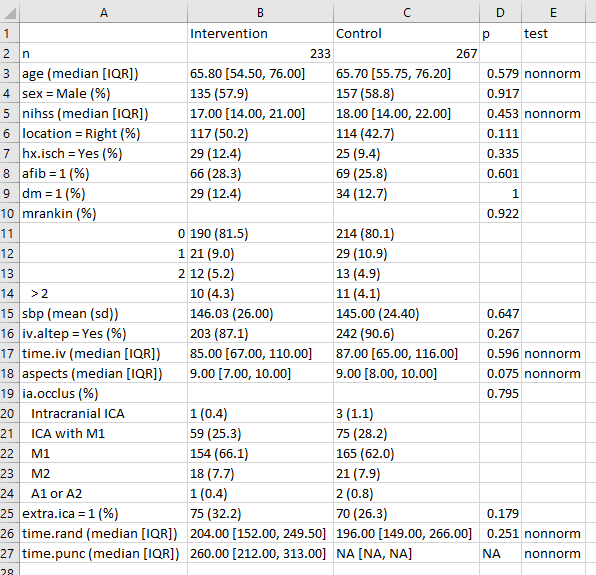
\includegraphics[width=0.9\linewidth]{images/fs-table1inExcel}

And from here, I can either drop it directly into Word, or present it as
is, or start tweaking it to meet formatting needs.

\subsection{Approach B: Produce the Table so you can cut and paste
it}\label{approach-b-produce-the-table-so-you-can-cut-and-paste-it}

\begin{Shaded}
\begin{Highlighting}[]
\KeywordTok{print}\NormalTok{(att2, }
      \DataTypeTok{nonnormal =} \KeywordTok{c}\NormalTok{(}\StringTok{"age"}\NormalTok{, }\StringTok{"nihss"}\NormalTok{, }\StringTok{"time.iv"}\NormalTok{, }\StringTok{"aspects"}\NormalTok{, }\StringTok{"time.rand"}\NormalTok{),}
      \DataTypeTok{exact =} \KeywordTok{c}\NormalTok{(}\StringTok{"location"}\NormalTok{, }\StringTok{"mrankin"}\NormalTok{),}
      \DataTypeTok{quote =} \OtherTok{TRUE}\NormalTok{, }\DataTypeTok{noSpaces =} \OtherTok{TRUE}\NormalTok{)}
\end{Highlighting}
\end{Shaded}

This will look like a mess by itself, but if you:

\begin{enumerate}
\def\labelenumi{\arabic{enumi}.}
\tightlist
\item
  copy and paste that mess into Excel
\item
  select Text to Columns from the Data menu
\item
  select Delimited, then Space and select Treat consecutive delimiters
  as one
\end{enumerate}

you should get something usable again.

Or, in Word,

\begin{enumerate}
\def\labelenumi{\arabic{enumi}.}
\tightlist
\item
  insert the text
\item
  select the text with your mouse
\item
  select Insert \ldots{} Table \ldots{} Convert Text to Table
\item
  place a quotation mark in the ``Other'' area under Separate text at
  \ldots{}
\end{enumerate}

After dropping blank columns, the result looks pretty good.

\section{A Controlled Biological Experiment - The Blood-Brain
Barrier}\label{a-controlled-biological-experiment---the-blood-brain-barrier}

My source for the data and the following explanatory paragraph is page
307 from \citet{RamseySchafer2002}. The original data come from
\citet{Barnett1995}.

\begin{quote}
The human brain (and that of rats, coincidentally) is protected from the
bacteria and toxins that course through the bloodstream by something
called the blood-brain barrier. After a method of disrupting the barrier
was developed, researchers tested this new mechanism, as follows. A
series of 34 rats were inoculated with human lung cancer cells to induce
brain tumors. After 9-11 days they were infused with either the barrier
disruption (BD) solution or, as a control, a normal saline (NS)
solution. Fifteen minutes later, the rats received a standard dose of a
particular therapeutic antibody (L6-F(ab')2. The key measure of the
effectiveness of transmission across the brain-blood barrier is the
ratio of the antibody concentration in the brain tumor to the antibody
concentration in normal tissue outside the brain. The rats were then
sacrificed, and the amounts of antibody in the brain tumor and in normal
tissue from the liver were measured. The study's primary objective is to
determine whether the antibody concentration in the tumor increased when
the blood-barrier disruption infusion was given, and if so, by how much?
\end{quote}

\section{\texorpdfstring{The \texttt{bloodbrain.csv}
file}{The bloodbrain.csv file}}\label{the-bloodbrain.csv-file}

Consider the data, available on the Data and Code page of
\href{https://github.com/THOMASELOVE/432-2018}{our course website} in
the \texttt{bloodbrain.csv} file, which includes the following
variables:

\begin{longtable}[]{@{}rl@{}}
\toprule
\begin{minipage}[b]{0.12\columnwidth}\raggedleft\strut
Variable\strut
\end{minipage} & \begin{minipage}[b]{0.59\columnwidth}\raggedright\strut
Description\strut
\end{minipage}\tabularnewline
\midrule
\endhead
\begin{minipage}[t]{0.12\columnwidth}\raggedleft\strut
\texttt{case}\strut
\end{minipage} & \begin{minipage}[t]{0.59\columnwidth}\raggedright\strut
identification number for the rat (1 - 34)\strut
\end{minipage}\tabularnewline
\begin{minipage}[t]{0.12\columnwidth}\raggedleft\strut
\texttt{brain}\strut
\end{minipage} & \begin{minipage}[t]{0.59\columnwidth}\raggedright\strut
an outcome: Brain tumor antibody count (per gram)\strut
\end{minipage}\tabularnewline
\begin{minipage}[t]{0.12\columnwidth}\raggedleft\strut
\texttt{liver}\strut
\end{minipage} & \begin{minipage}[t]{0.59\columnwidth}\raggedright\strut
an outcome: Liver antibody count (per gram)\strut
\end{minipage}\tabularnewline
\begin{minipage}[t]{0.12\columnwidth}\raggedleft\strut
\texttt{tlratio}\strut
\end{minipage} & \begin{minipage}[t]{0.59\columnwidth}\raggedright\strut
an outcome: tumor / liver concentration ratio\strut
\end{minipage}\tabularnewline
\begin{minipage}[t]{0.12\columnwidth}\raggedleft\strut
\texttt{solution}\strut
\end{minipage} & \begin{minipage}[t]{0.59\columnwidth}\raggedright\strut
the treatment: BD (barrier disruption) or NS (normal saline)\strut
\end{minipage}\tabularnewline
\begin{minipage}[t]{0.12\columnwidth}\raggedleft\strut
\texttt{sactime}\strut
\end{minipage} & \begin{minipage}[t]{0.59\columnwidth}\raggedright\strut
a design variable: Sacrifice time (hours; either 0.5, 3, 24 or 72)\strut
\end{minipage}\tabularnewline
\begin{minipage}[t]{0.12\columnwidth}\raggedleft\strut
\texttt{postin}\strut
\end{minipage} & \begin{minipage}[t]{0.59\columnwidth}\raggedright\strut
covariate: Days post-inoculation of lung cancer cells (9, 10 or
11)\strut
\end{minipage}\tabularnewline
\begin{minipage}[t]{0.12\columnwidth}\raggedleft\strut
\texttt{sex}\strut
\end{minipage} & \begin{minipage}[t]{0.59\columnwidth}\raggedright\strut
covariate: M or F\strut
\end{minipage}\tabularnewline
\begin{minipage}[t]{0.12\columnwidth}\raggedleft\strut
\texttt{wt.init}\strut
\end{minipage} & \begin{minipage}[t]{0.59\columnwidth}\raggedright\strut
covariate: Initial weight (grams)\strut
\end{minipage}\tabularnewline
\begin{minipage}[t]{0.12\columnwidth}\raggedleft\strut
\texttt{wt.loss}\strut
\end{minipage} & \begin{minipage}[t]{0.59\columnwidth}\raggedright\strut
covariate: Weight loss (grams)\strut
\end{minipage}\tabularnewline
\begin{minipage}[t]{0.12\columnwidth}\raggedleft\strut
\texttt{wt.tumor}\strut
\end{minipage} & \begin{minipage}[t]{0.59\columnwidth}\raggedright\strut
covariate: Tumor weight (10\textsuperscript{-4} grams)\strut
\end{minipage}\tabularnewline
\bottomrule
\end{longtable}

And here's what the data look like in R.

\begin{Shaded}
\begin{Highlighting}[]
\NormalTok{bloodbrain}
\end{Highlighting}
\end{Shaded}

\begin{verbatim}
# A tibble: 34 x 11
    case  brain   liver tlratio solution sactime postin sex   wt.init
   <int>  <int>   <int>   <dbl> <fct>      <dbl>  <int> <fct>   <int>
 1     1  41081 1456164  0.0282 BD         0.500     10 F         239
 2     2  44286 1602171  0.0276 BD         0.500     10 F         225
 3     3 102926 1601936  0.0642 BD         0.500     10 F         224
 4     4  25927 1776411  0.0146 BD         0.500     10 F         184
 5     5  42643 1351184  0.0316 BD         0.500     10 F         250
 6     6  31342 1790863  0.0175 NS         0.500     10 F         196
 7     7  22815 1633386  0.0140 NS         0.500     10 F         200
 8     8  16629 1618757  0.0103 NS         0.500     10 F         273
 9     9  22315 1567602  0.0142 NS         0.500     10 F         216
10    10  77961 1060057  0.0735 BD         3.00      10 F         267
# ... with 24 more rows, and 2 more variables: wt.loss <dbl>, wt.tumor
#   <int>
\end{verbatim}

\section{\texorpdfstring{A Table 1 for
\texttt{bloodbrain}}{A Table 1 for bloodbrain}}\label{a-table-1-for-bloodbrain}

\citet{Barnett1995} did not provide a Table 1 for these data, so let's
build one to compare the two \texttt{solutions} (\texttt{BD} vs.
\texttt{NS}) on the covariates and outcomes, plus the natural logarithm
of the tumor/liver concentration ratio (\texttt{tlratio}). We'll opt to
treat the sacrifice time (\texttt{sactime}) and the days
post-inoculation of lung cancer cells (\texttt{postin}) as categorical
rather than quantitative variables.

\begin{Shaded}
\begin{Highlighting}[]
\NormalTok{bloodbrain <-}\StringTok{ }\NormalTok{bloodbrain }\OperatorTok
\StringTok{    }\KeywordTok{mutate}\NormalTok{(}\DataTypeTok{logTL =} \KeywordTok{log}\NormalTok{(tlratio))}

\KeywordTok{dput}\NormalTok{(}\KeywordTok{names}\NormalTok{(bloodbrain))}
\end{Highlighting}
\end{Shaded}

\begin{verbatim}
c("case", "brain", "liver", "tlratio", "solution", "sactime", 
"postin", "sex", "wt.init", "wt.loss", "wt.tumor", "logTL")
\end{verbatim}

OK - there's the list of variables we'll need. I'll put the outcomes at
the bottom of the table.

\begin{Shaded}
\begin{Highlighting}[]
\NormalTok{bb.vars <-}\StringTok{ }\KeywordTok{c}\NormalTok{(}\StringTok{"sactime"}\NormalTok{, }\StringTok{"postin"}\NormalTok{, }\StringTok{"sex"}\NormalTok{, }\StringTok{"wt.init"}\NormalTok{, }\StringTok{"wt.loss"}\NormalTok{, }
             \StringTok{"wt.tumor"}\NormalTok{, }\StringTok{"brain"}\NormalTok{, }\StringTok{"liver"}\NormalTok{, }\StringTok{"tlratio"}\NormalTok{, }\StringTok{"logTL"}\NormalTok{)}

\NormalTok{bb.factors <-}\StringTok{ }\KeywordTok{c}\NormalTok{(}\StringTok{"sactime"}\NormalTok{, }\StringTok{"sex"}\NormalTok{, }\StringTok{"postin"}\NormalTok{)}

\NormalTok{bb.att1 <-}\StringTok{ }\KeywordTok{CreateTableOne}\NormalTok{(}\DataTypeTok{data =}\NormalTok{ bloodbrain,}
                          \DataTypeTok{vars =}\NormalTok{ bb.vars,}
                          \DataTypeTok{factorVars =}\NormalTok{ bb.factors,}
                          \DataTypeTok{strata =} \KeywordTok{c}\NormalTok{(}\StringTok{"solution"}\NormalTok{))}
\KeywordTok{summary}\NormalTok{(bb.att1)}
\end{Highlighting}
\end{Shaded}

\begin{verbatim}

     ### Summary of continuous variables ###

solution: BD
          n miss p.miss   mean    sd median    p25   p75    min   max
wt.init  17    0      0    243 3e+01  2e+02  2e+02 3e+02  2e+02 3e+02
wt.loss  17    0      0      3 5e+00  4e+00  1e+00 6e+00 -5e+00 1e+01
wt.tumor 17    0      0    157 8e+01  2e+02  1e+02 2e+02  2e+01 4e+02
brain    17    0      0  56043 3e+04  5e+04  4e+04 8e+04  6e+03 1e+05
liver    17    0      0 672577 7e+05  6e+05  2e+04 1e+06  2e+03 2e+06
tlratio  17    0      0      2 3e+00  1e-01  6e-02 3e+00  1e-02 9e+00
logTL    17    0      0     -1 2e+00 -2e+00 -3e+00 1e+00 -4e+00 2e+00
          skew kurt
wt.init  -0.39  0.7
wt.loss  -0.10  0.2
wt.tumor  0.53  1.0
brain     0.29 -0.6
liver     0.35 -1.7
tlratio   1.58  1.7
logTL     0.08 -1.7
-------------------------------------------------------- 
solution: NS
          n miss p.miss   mean    sd median    p25    p75    min   max
wt.init  17    0      0    240 3e+01  2e+02  2e+02  3e+02  2e+02 3e+02
wt.loss  17    0      0      4 4e+00  3e+00  2e+00  7e+00 -4e+00 1e+01
wt.tumor 17    0      0    209 1e+02  2e+02  2e+02  3e+02  3e+01 5e+02
brain    17    0      0  23887 1e+04  2e+04  1e+04  3e+04  1e+03 5e+04
liver    17    0      0 664975 7e+05  7e+05  2e+04  1e+06  9e+02 2e+06
tlratio  17    0      0      1 2e+00  5e-02  3e-02  9e-01  1e-02 7e+00
logTL    17    0      0     -2 2e+00 -3e+00 -3e+00 -7e-02 -5e+00 2e+00
          skew  kurt
wt.init   0.33 -0.48
wt.loss  -0.09  0.08
wt.tumor  0.63  0.77
brain     0.30 -0.35
liver     0.40 -1.56
tlratio   2.27  4.84
logTL     0.27 -1.61

p-values
             pNormal  pNonNormal
wt.init  0.807308940 0.641940278
wt.loss  0.683756156 0.876749808
wt.tumor 0.151510151 0.190482094
brain    0.001027678 0.002579901
liver    0.974853609 0.904045603
tlratio  0.320501715 0.221425879
logTL    0.351633525 0.221425879

Standardize mean differences
             1 vs 2
wt.init  0.08435244
wt.loss  0.14099823
wt.tumor 0.50397184
brain    1.23884159
liver    0.01089667
tlratio  0.34611465
logTL    0.32420504

=======================================================================================

     ### Summary of categorical variables ### 

solution: BD
     var  n miss p.miss level freq percent cum.percent
 sactime 17    0    0.0   0.5    5    29.4        29.4
                            3    4    23.5        52.9
                           24    4    23.5        76.5
                           72    4    23.5       100.0
                                                      
  postin 17    0    0.0     9    1     5.9         5.9
                           10   14    82.4        88.2
                           11    2    11.8       100.0
                                                      
     sex 17    0    0.0     F   13    76.5        76.5
                            M    4    23.5       100.0
                                                      
-------------------------------------------------------- 
solution: NS
     var  n miss p.miss level freq percent cum.percent
 sactime 17    0    0.0   0.5    4    23.5        23.5
                            3    5    29.4        52.9
                           24    4    23.5        76.5
                           72    4    23.5       100.0
                                                      
  postin 17    0    0.0     9    2    11.8        11.8
                           10   13    76.5        88.2
                           11    2    11.8       100.0
                                                      
     sex 17    0    0.0     F   13    76.5        76.5
                            M    4    23.5       100.0
                                                      

p-values
          pApprox pExact
sactime 0.9739246      1
postin  0.8309504      1
sex     1.0000000      1

Standardize mean differences
           1 vs 2
sactime 0.1622214
postin  0.2098877
sex     0.0000000
\end{verbatim}

\subsection{\texorpdfstring{Generate final Table 1 for
\texttt{bloodbrain}}{Generate final Table 1 for bloodbrain}}\label{generate-final-table-1-for-bloodbrain}

I'll choose to treat \texttt{tlratio} as non-Normal, but otherwise, use
t tests.

\begin{Shaded}
\begin{Highlighting}[]
\KeywordTok{print}\NormalTok{(bb.att1, }\DataTypeTok{nonnormal =} \KeywordTok{c}\NormalTok{(}\StringTok{"tlratio"}\NormalTok{, }\StringTok{"logTL"}\NormalTok{))}
\end{Highlighting}
\end{Shaded}

\begin{verbatim}
                        Stratified by solution
                         BD                      NS                      
  n                             17                      17               
  sactime (%)                                                            
     0.5                         5 (29.4)                4 (23.5)        
     3                           4 (23.5)                5 (29.4)        
     24                          4 (23.5)                4 (23.5)        
     72                          4 (23.5)                4 (23.5)        
  postin (%)                                                             
     9                           1 ( 5.9)                2 (11.8)        
     10                         14 (82.4)               13 (76.5)        
     11                          2 (11.8)                2 (11.8)        
  sex = M (%)                    4 (23.5)                4 (23.5)        
  wt.init (mean (sd))       242.82 (27.23)          240.47 (28.54)       
  wt.loss (mean (sd))         3.34 (4.68)             3.94 (3.88)        
  wt.tumor (mean (sd))      157.29 (84.00)          208.53 (116.68)      
  brain (mean (sd))       56043.41 (33675.40)     23887.18 (14610.53)    
  liver (mean (sd))      672577.35 (694479.58)   664975.47 (700773.13)   
  tlratio (median [IQR])      0.12 [0.06, 2.84]       0.05 [0.03, 0.94]  
  logTL (median [IQR])       -2.10 [-2.74, 1.04]     -2.95 [-3.41, -0.07]
                        Stratified by solution
                         p      test   
  n                                    
  sactime (%)             0.974        
     0.5                               
     3                                 
     24                                
     72                                
  postin (%)              0.831        
     9                                 
     10                                
     11                                
  sex = M (%)             1.000        
  wt.init (mean (sd))     0.807        
  wt.loss (mean (sd))     0.684        
  wt.tumor (mean (sd))    0.152        
  brain (mean (sd))       0.001        
  liver (mean (sd))       0.975        
  tlratio (median [IQR])  0.221 nonnorm
  logTL (median [IQR])    0.221 nonnorm
\end{verbatim}

Or, we can get an Excel-readable version, using

\begin{Shaded}
\begin{Highlighting}[]
\NormalTok{bb.t1 <-}\StringTok{ }\KeywordTok{print}\NormalTok{(bb.att1, }\DataTypeTok{nonnormal =} \KeywordTok{c}\NormalTok{(}\StringTok{"tlratio"}\NormalTok{, }\StringTok{"logTL"}\NormalTok{), }\DataTypeTok{quote =} \OtherTok{FALSE}\NormalTok{,}
               \DataTypeTok{noSpaces =} \OtherTok{TRUE}\NormalTok{, }\DataTypeTok{printToggle =} \OtherTok{FALSE}\NormalTok{)}

\KeywordTok{write.csv}\NormalTok{(bb.t1, }\DataTypeTok{file =} \StringTok{"bb-table1.csv"}\NormalTok{)}
\end{Highlighting}
\end{Shaded}

which, when dropped into Excel, will look like this:

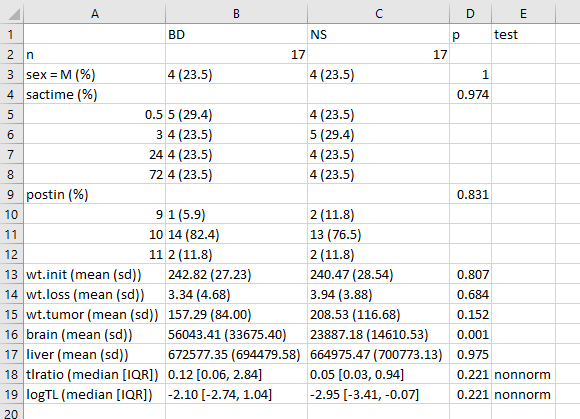
\includegraphics[width=0.9\linewidth]{images/bb-table1inExcel}

One thing I would definitely clean up here, in practice, is to change
the presentation of the \emph{p} value for \texttt{sex} from 1 to
\textgreater{} 0.99, or just omit it altogether. I'd also drop the
\texttt{computer-ese} where possible, add units for the measures, round
\textbf{a lot}, identify the outcomes carefully, and use notes to
indicate deviations from the main approach.

\subsection{A More Finished Version (after Cleanup in
Word)}\label{a-more-finished-version-after-cleanup-in-word}

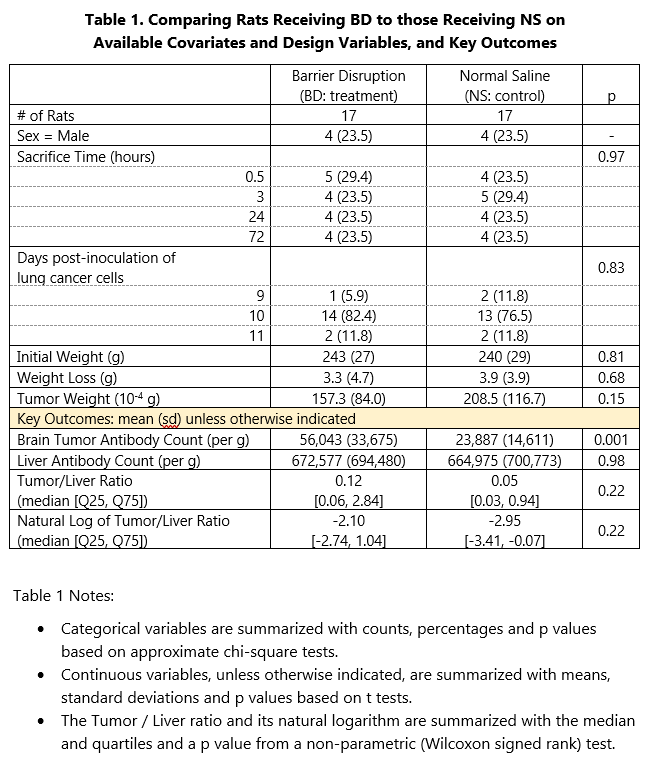
\includegraphics[width=0.95\linewidth]{images/bb-table1inWord}

\chapter{Linear Regression on a small SMART data
set}\label{linear-regression-on-a-small-smart-data-set}

\section{BRFSS and SMART}\label{brfss-and-smart}

The Centers for Disease Control analyzes Behavioral Risk Factor
Surveillance System (BRFSS) survey data for specific metropolitan and
micropolitan statistical areas (MMSAs) in a program called the
\href{https://www.cdc.gov/brfss/smart/Smart_data.htm}{Selected
Metropolitan/Micropolitan Area Risk Trends of BRFSS} (SMART BRFSS.)

In this work, we will focus on
\href{https://www.cdc.gov/brfss/smart/smart_2016.html}{data from the
2016 SMART}, and in particular on data from the Cleveland-Elyria, OH,
Metropolitan Statistical Area. The purpose of this survey is to provide
localized health information that can help public health practitioners
identify local emerging health problems, plan and evaluate local
responses, and efficiently allocate resources to specific needs.

\subsection{Key resources}\label{key-resources}

\begin{itemize}
\tightlist
\item
  the full data are available in the form of the 2016 SMART BRFSS MMSA
  Data, found in a zipped
  \href{https://www.cdc.gov/brfss/smart/2016/MMSA2016_XPT.zip}{SAS
  Transport Format} file. The data were released in August 2017.
\item
  the
  \href{https://www.cdc.gov/brfss/smart/2016/mmsa_varlayout_16.pdf}{MMSA
  Variable Layout PDF} which simply lists the variables included in the
  data file
\item
  the
  \href{https://www.cdc.gov/brfss/annual_data/2016/pdf/2016_calculated_variables_version4.pdf}{Calculated
  Variables PDF} which describes the risk factors by data variable names
  - there is also an
  \href{https://www.cdc.gov/brfss/annual_data/2016/Summary_Matrix_16.html}{online
  summary matrix of these calculated variables}, as well.
\item
  the lengthy
  \href{https://www.cdc.gov/brfss/questionnaires/pdf-ques/2016_BRFSS_Questionnaire_FINAL.pdf}{2016
  Survey Questions PDF} which lists all questions asked as part of the
  BRFSS in 2016
\item
  the enormous
  \href{https://www.cdc.gov/brfss/annual_data/2016/pdf/codebook16_llcp.pdf}{Codebook
  for the 2016 BRFSS Survey PDF} which identifies the variables by name
  for us.
\end{itemize}

Later this term, we'll use all of those resources to help construct a
more complete data set than we'll study today. I'll also demonstrate how
I built the \texttt{smartcle1} data set that we'll use in this Chapter.

\section{\texorpdfstring{The \texttt{smartcle1} data:
Cookbook}{The smartcle1 data: Cookbook}}\label{the-smartcle1-data-cookbook}

The \texttt{smartcle1.csv} data file available on the Data and Code page
of \href{https://github.com/THOMASELOVE/432-2018}{our website} describes
information on 11 variables for 1036 respondents to the BRFSS 2016, who
live in the Cleveland-Elyria, OH, Metropolitan Statistical Area. The
variables in the \texttt{smartcle1.csv} file are listed below, along
with (in some cases) the BRFSS items that generate these responses.

\begin{longtable}[]{@{}rl@{}}
\toprule
\begin{minipage}[b]{0.14\columnwidth}\raggedleft\strut
Variable\strut
\end{minipage} & \begin{minipage}[b]{0.74\columnwidth}\raggedright\strut
Description\strut
\end{minipage}\tabularnewline
\midrule
\endhead
\begin{minipage}[t]{0.14\columnwidth}\raggedleft\strut
\texttt{SEQNO}\strut
\end{minipage} & \begin{minipage}[t]{0.74\columnwidth}\raggedright\strut
respondent identification number (all begin with 2016)\strut
\end{minipage}\tabularnewline
\begin{minipage}[t]{0.14\columnwidth}\raggedleft\strut
\texttt{physhealth}\strut
\end{minipage} & \begin{minipage}[t]{0.74\columnwidth}\raggedright\strut
Now thinking about your physical health, which includes physical illness
and injury, for how many days during the past 30 days was your physical
health not good?\strut
\end{minipage}\tabularnewline
\begin{minipage}[t]{0.14\columnwidth}\raggedleft\strut
\texttt{menthealth}\strut
\end{minipage} & \begin{minipage}[t]{0.74\columnwidth}\raggedright\strut
Now thinking about your mental health, which includes stress,
depression, and problems with emotions, for how many days during the
past 30 days was your mental health not good?\strut
\end{minipage}\tabularnewline
\begin{minipage}[t]{0.14\columnwidth}\raggedleft\strut
\texttt{poorhealth}\strut
\end{minipage} & \begin{minipage}[t]{0.74\columnwidth}\raggedright\strut
During the past 30 days, for about how many days did poor physical or
mental health keep you from doing your usual activities, such as
self-care, work, or recreation?\strut
\end{minipage}\tabularnewline
\begin{minipage}[t]{0.14\columnwidth}\raggedleft\strut
\texttt{genhealth}\strut
\end{minipage} & \begin{minipage}[t]{0.74\columnwidth}\raggedright\strut
Would you say that in general, your health is \ldots{} (five categories:
Excellent, Very Good, Good, Fair or Poor)\strut
\end{minipage}\tabularnewline
\begin{minipage}[t]{0.14\columnwidth}\raggedleft\strut
\texttt{bmi}\strut
\end{minipage} & \begin{minipage}[t]{0.74\columnwidth}\raggedright\strut
Body mass index, in kg/m\textsuperscript{2}\strut
\end{minipage}\tabularnewline
\begin{minipage}[t]{0.14\columnwidth}\raggedleft\strut
\texttt{female}\strut
\end{minipage} & \begin{minipage}[t]{0.74\columnwidth}\raggedright\strut
Sex, 1 = female, 0 = male\strut
\end{minipage}\tabularnewline
\begin{minipage}[t]{0.14\columnwidth}\raggedleft\strut
\texttt{internet30}\strut
\end{minipage} & \begin{minipage}[t]{0.74\columnwidth}\raggedright\strut
Have you used the internet in the past 30 days? (1 = yes, 0 = no)\strut
\end{minipage}\tabularnewline
\begin{minipage}[t]{0.14\columnwidth}\raggedleft\strut
\texttt{exerany}\strut
\end{minipage} & \begin{minipage}[t]{0.74\columnwidth}\raggedright\strut
During the past month, other than your regular job, did you participate
in any physical activities or exercises such as running, calisthenics,
golf, gardening, or walking for exercise? (1 = yes, 0 = no)\strut
\end{minipage}\tabularnewline
\begin{minipage}[t]{0.14\columnwidth}\raggedleft\strut
\texttt{sleephrs}\strut
\end{minipage} & \begin{minipage}[t]{0.74\columnwidth}\raggedright\strut
On average, how many hours of sleep do you get in a 24-hour
period?\strut
\end{minipage}\tabularnewline
\begin{minipage}[t]{0.14\columnwidth}\raggedleft\strut
\texttt{alcdays}\strut
\end{minipage} & \begin{minipage}[t]{0.74\columnwidth}\raggedright\strut
How many days during the past 30 days did you have at least one drink of
any alcoholic beverage such as beer, wine, a malt beverage or
liquor?\strut
\end{minipage}\tabularnewline
\bottomrule
\end{longtable}

\begin{Shaded}
\begin{Highlighting}[]
\KeywordTok{str}\NormalTok{(smartcle1)}
\end{Highlighting}
\end{Shaded}

\begin{verbatim}
Classes 'tbl_df', 'tbl' and 'data.frame':   1036 obs. of  11 variables:
 $ SEQNO     : num  2.02e+09 2.02e+09 2.02e+09 2.02e+09 2.02e+09 ...
 $ physhealth: int  0 0 1 0 5 4 2 2 0 0 ...
 $ menthealth: int  0 0 5 0 0 18 0 3 0 0 ...
 $ poorhealth: int  NA NA 0 NA 0 6 0 0 NA NA ...
 $ genhealth : Factor w/ 5 levels "1_Excellent",..: 2 1 2 3 1 2 3 3 2 3 ...
 $ bmi       : num  26.7 23.7 26.9 21.7 24.1 ...
 $ female    : int  1 0 0 1 0 0 1 1 0 0 ...
 $ internet30: int  1 1 1 1 1 1 1 1 1 1 ...
 $ exerany   : int  1 1 0 1 1 1 1 1 1 0 ...
 $ sleephrs  : int  6 6 8 9 7 5 9 7 7 7 ...
 $ alcdays   : int  1 4 4 3 2 28 4 2 4 25 ...
\end{verbatim}

\subsection{Omitting Missing Observations: Complete-Case
Analyses}\label{omitting-missing-observations-complete-case-analyses}

For the purpose of fitting our first few models, we will eliminate the
missingness problem, and look only at the \emph{complete cases} in our
\texttt{smartcle1} data.

To inspect the missingness in our data, we might consider using the
\texttt{skim} function from the \texttt{skimr} package. We'll exclude
the respondent identifier code (\texttt{SEQNO}) from this summary as
uninteresting. In this case, we'll use the \texttt{skim\_with} command
to set some options that will make this book work a bit more
effectively, by eliminating the spark graphs that we'll demonstrate in
class.

\begin{Shaded}
\begin{Highlighting}[]
\KeywordTok{skim_with}\NormalTok{(}\DataTypeTok{numeric =} \KeywordTok{list}\NormalTok{(}\DataTypeTok{hist =} \OtherTok{NULL}\NormalTok{), }\DataTypeTok{ts =} \KeywordTok{list}\NormalTok{(}\DataTypeTok{line_graph =} \OtherTok{NULL}\NormalTok{))}

\NormalTok{smartcle1 }\OperatorTok\StringTok{ }\KeywordTok{skim}\NormalTok{(}\OperatorTok{-}\NormalTok{SEQNO)}
\end{Highlighting}
\end{Shaded}

\begin{verbatim}
Skim summary statistics
 n obs: 1036 
 n variables: 11 

Variable type: factor 
  variable missing complete    n n_unique
 genhealth       3     1033 1036        5
                             top_counts ordered
 2_V: 350, 3_G: 344, 1_E: 173, 4_F: 122   FALSE

Variable type: integer 
   variable missing complete    n mean   sd p0 p25 median p75 p100
    alcdays      46      990 1036 4.65 8.05  0   0      1   4   30
    exerany       3     1033 1036 0.76 0.43  0   1      1   1    1
     female       0     1036 1036 0.6  0.49  0   0      1   1    1
 internet30       6     1030 1036 0.81 0.39  0   1      1   1    1
 menthealth      11     1025 1036 2.72 6.82  0   0      0   2   30
 physhealth      17     1019 1036 3.97 8.67  0   0      0   2   30
 poorhealth     543      493 1036 4.07 8.09  0   0      0   3   30
   sleephrs       8     1028 1036 7.02 1.53  1   6      7   8   20
     hist
 <U+2587><U+2582><U+2581><U+2581><U+2581><U+2581><U+2581><U+2581>
 <U+2582><U+2581><U+2581><U+2581><U+2581><U+2581><U+2581><U+2587>
 <U+2585><U+2581><U+2581><U+2581><U+2581><U+2581><U+2581><U+2587>
 <U+2582><U+2581><U+2581><U+2581><U+2581><U+2581><U+2581><U+2587>
 <U+2587><U+2581><U+2581><U+2581><U+2581><U+2581><U+2581><U+2581>
 <U+2587><U+2581><U+2581><U+2581><U+2581><U+2581><U+2581><U+2581>
 <U+2587><U+2581><U+2581><U+2581><U+2581><U+2581><U+2581><U+2581>
 <U+2581><U+2581><U+2587><U+2581><U+2581><U+2581><U+2581><U+2581>

Variable type: numeric 
 variable missing complete    n  mean   sd    p0  p25 median   p75  p100
      bmi      84      952 1036 27.89 6.47 12.71 23.7  26.68 30.53 66.06
\end{verbatim}

Now, we'll create a new tibble called \texttt{smartcle2} which contains
every variable except \texttt{poorhealth}, and which includes all
respondents with complete data on the variables (other than
\texttt{poorhealth}). We'll store those observations with complete data
in the \texttt{smartcle2} tibble.

\begin{Shaded}
\begin{Highlighting}[]
\NormalTok{smartcle2 <-}\StringTok{ }\NormalTok{smartcle1 }\OperatorTok\StringTok{ }
\StringTok{    }\KeywordTok{select}\NormalTok{(}\OperatorTok{-}\NormalTok{poorhealth) }\OperatorTok
\StringTok{    }\KeywordTok{filter}\NormalTok{(}\KeywordTok{complete.cases}\NormalTok{(.))}

\NormalTok{smartcle2}
\end{Highlighting}
\end{Shaded}

\begin{verbatim}
# A tibble: 896 x 10
     SEQNO physhealth menthealth genhealth   bmi female internet30 exerany
     <dbl>      <int>      <int> <fct>     <dbl>  <int>      <int>   <int>
 1  2.02e9          0          0 2_VeryGo~  26.7      1          1       1
 2  2.02e9          0          0 1_Excell~  23.7      0          1       1
 3  2.02e9          1          5 2_VeryGo~  26.9      0          1       0
 4  2.02e9          0          0 3_Good     21.7      1          1       1
 5  2.02e9          5          0 1_Excell~  24.1      0          1       1
 6  2.02e9          4         18 2_VeryGo~  27.6      0          1       1
 7  2.02e9          2          0 3_Good     25.7      1          1       1
 8  2.02e9          2          3 3_Good     28.5      1          1       1
 9  2.02e9          0          0 2_VeryGo~  28.6      0          1       1
10  2.02e9          0          0 3_Good     23.1      0          1       0
# ... with 886 more rows, and 2 more variables: sleephrs <int>, alcdays
#   <int>
\end{verbatim}

Note that there are only 896 respondents with \textbf{complete} data on
the 10 variables (excluding \texttt{poorhealth}) in the
\texttt{smartcle2} tibble, as compared to our original
\texttt{smartcle1} data which described 1036 respondents and 11
variables, but with lots of missing data.

\section{\texorpdfstring{Model A: Predicting
\texttt{physhealth}}{Model A: Predicting physhealth}}\label{model-a-predicting-physhealth}

We'll begin by investigating the problem of predicting
\texttt{physhealth}, at first with just two predictor variables:
\texttt{exerany} and \texttt{bmi}, in our new \texttt{smartcle2} data
set.

\subsection{Graphing The Data}\label{graphing-the-data}

We'll start by building an exploratory figure to show the relationship
between \texttt{bmi} and \texttt{physhealth} within each of the two
\texttt{exerany} groups.

\begin{Shaded}
\begin{Highlighting}[]
\KeywordTok{ggplot}\NormalTok{(smartcle2, }\KeywordTok{aes}\NormalTok{(}\DataTypeTok{x =}\NormalTok{ bmi, }\DataTypeTok{y =}\NormalTok{ physhealth, }\DataTypeTok{group =}\NormalTok{ exerany, }\DataTypeTok{color =} \KeywordTok{factor}\NormalTok{(exerany))) }\OperatorTok{+}
\StringTok{    }\KeywordTok{geom_point}\NormalTok{() }\OperatorTok{+}
\StringTok{    }\KeywordTok{geom_smooth}\NormalTok{(}\DataTypeTok{method =} \StringTok{"lm"}\NormalTok{, }\DataTypeTok{se =} \OtherTok{FALSE}\NormalTok{) }\OperatorTok{+}\StringTok{ }
\StringTok{    }\KeywordTok{theme_bw}\NormalTok{()}
\end{Highlighting}
\end{Shaded}

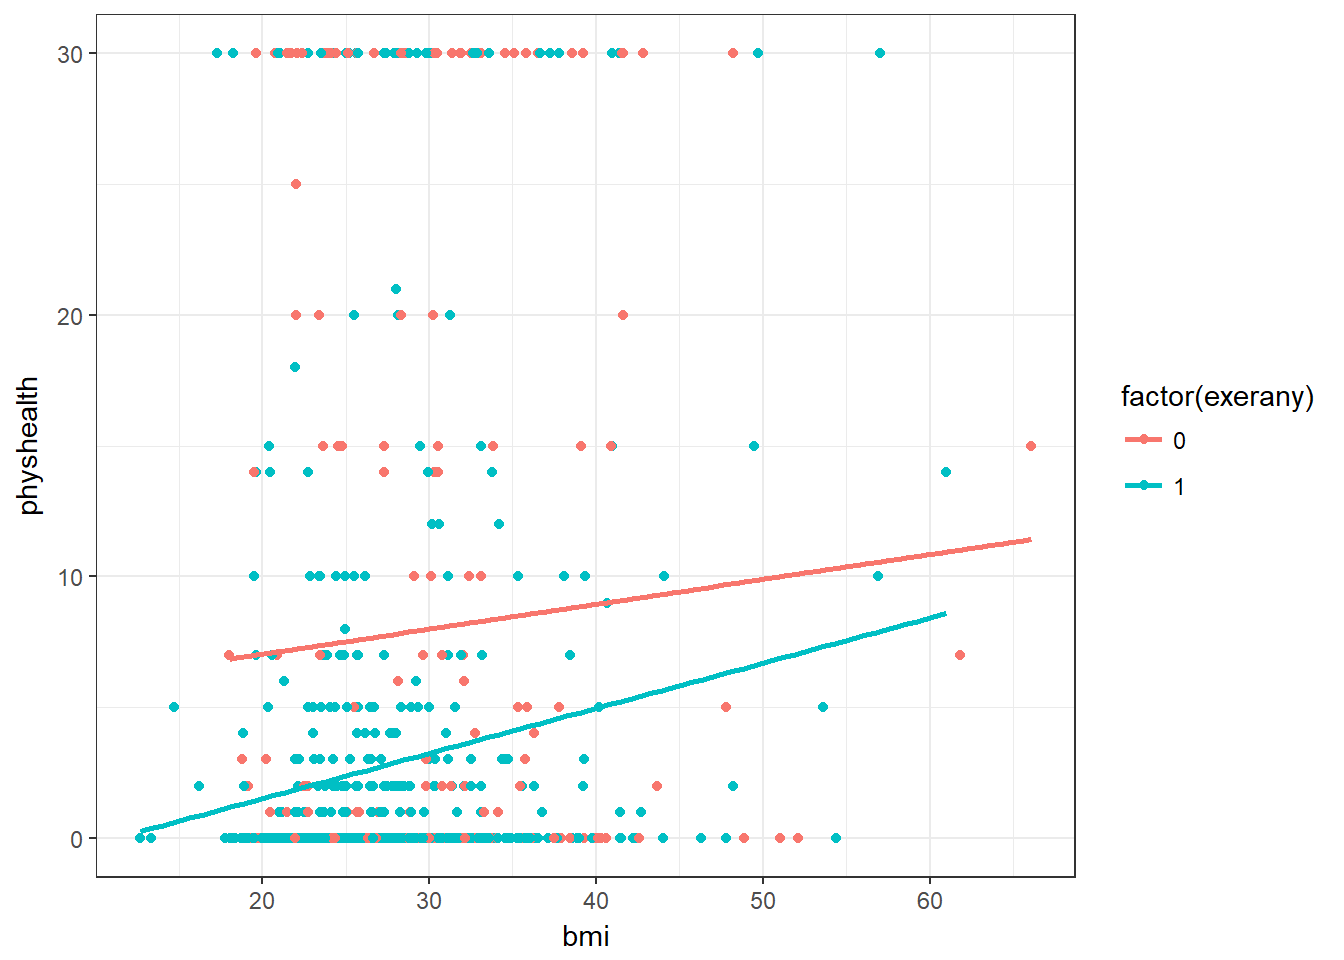
\includegraphics{bookdown-demo_files/figure-latex/gr_smartcle2_1_fig-1.pdf}

The figure \emph{could} be improved by separating the two groups into
facets.

\begin{Shaded}
\begin{Highlighting}[]
\KeywordTok{ggplot}\NormalTok{(smartcle2, }\KeywordTok{aes}\NormalTok{(}\DataTypeTok{x =}\NormalTok{ bmi, }\DataTypeTok{y =}\NormalTok{ physhealth, }\DataTypeTok{group =}\NormalTok{ exerany, }\DataTypeTok{color =} \KeywordTok{factor}\NormalTok{(exerany))) }\OperatorTok{+}
\StringTok{    }\KeywordTok{geom_point}\NormalTok{() }\OperatorTok{+}
\StringTok{    }\KeywordTok{geom_smooth}\NormalTok{(}\DataTypeTok{method =} \StringTok{"lm"}\NormalTok{, }\DataTypeTok{se =} \OtherTok{FALSE}\NormalTok{) }\OperatorTok{+}\StringTok{ }
\StringTok{    }\KeywordTok{theme_bw}\NormalTok{() }\OperatorTok{+}\StringTok{ }
\StringTok{    }\KeywordTok{guides}\NormalTok{(}\DataTypeTok{color =} \OtherTok{FALSE}\NormalTok{) }\OperatorTok{+}
\StringTok{    }\KeywordTok{facet_wrap}\NormalTok{(}\OperatorTok{~}\StringTok{ }\NormalTok{exerany)}
\end{Highlighting}
\end{Shaded}

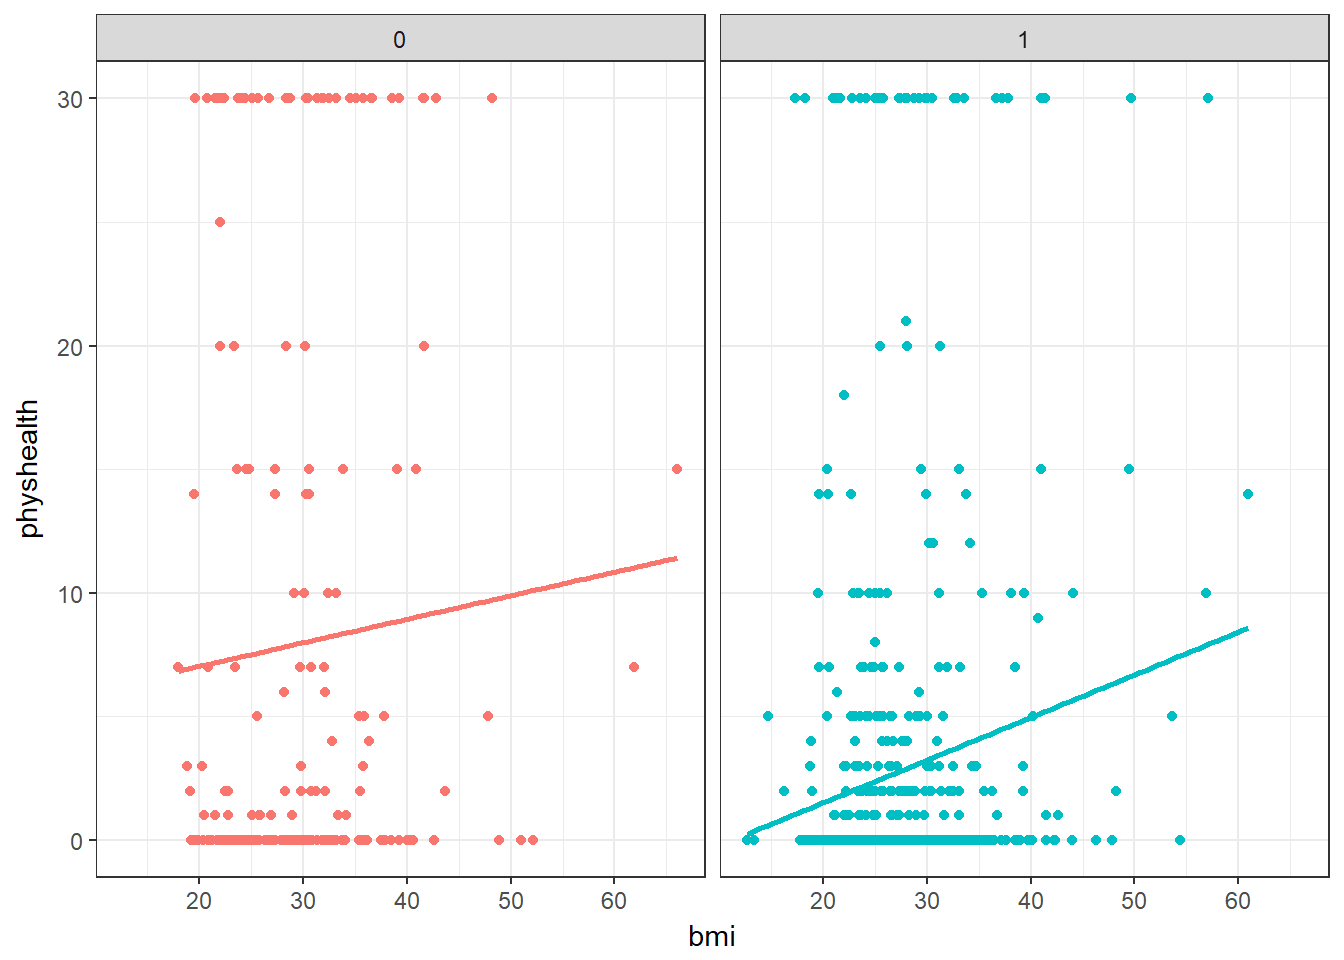
\includegraphics{bookdown-demo_files/figure-latex/gr_smartcle2_2_fig-1.pdf}

Now, what can we learn from these plots?

\begin{enumerate}
\def\labelenumi{\arabic{enumi}.}
\tightlist
\item
  Does \texttt{physhealth} look like a good candidate for a linear
  model?
\item
  Does there seem to be a meaningful difference in the slopes of the two
  fitted lines?
\item
  In what BMI range can we make a reasonable prediction of
  \texttt{physhealth}?
\end{enumerate}

\subsection{Building Model A}\label{building-model-a}

First, we'll fit a simple model describing the main effects but not the
interaction of \texttt{exerany} and \texttt{bmi}, without doing any of
the exploratory ground work we should do in advance.

\begin{Shaded}
\begin{Highlighting}[]
\NormalTok{modA <-}\StringTok{ }\KeywordTok{lm}\NormalTok{(physhealth }\OperatorTok{~}\StringTok{ }\NormalTok{exerany }\OperatorTok{*}\StringTok{ }\NormalTok{bmi, }\DataTypeTok{data =}\NormalTok{ smartcle2)}
\KeywordTok{glance}\NormalTok{(modA)}
\end{Highlighting}
\end{Shaded}

\begin{verbatim}
   r.squared adj.r.squared    sigma statistic     p.value df    logLik
1 0.07607716     0.0729698 8.318521  24.48286 3.14356e-15  4 -3167.527
       AIC      BIC deviance df.residual
1 6345.053 6369.043 61724.43         892
\end{verbatim}

\begin{Shaded}
\begin{Highlighting}[]
\KeywordTok{tidy}\NormalTok{(modA)}
\end{Highlighting}
\end{Shaded}

\begin{verbatim}
         term    estimate std.error  statistic    p.value
1 (Intercept)  5.13460484 2.3570652  2.1783890 0.02963831
2     exerany -7.06992980 2.8044237 -2.5209921 0.01187578
3         bmi  0.09527214 0.0772901  1.2326565 0.21802872
4 exerany:bmi  0.07732883 0.0944822  0.8184487 0.41331959
\end{verbatim}

\begin{Shaded}
\begin{Highlighting}[]
\KeywordTok{summary}\NormalTok{(modA)}
\end{Highlighting}
\end{Shaded}

\begin{verbatim}

Call:
lm(formula = physhealth ~ exerany * bmi, data = smartcle2)

Residuals:
     Min       1Q   Median       3Q      Max 
-10.0992  -3.4231  -2.3780  -0.9199  28.9493 

Coefficients:
            Estimate Std. Error t value Pr(>|t|)  
(Intercept)  5.13460    2.35707   2.178   0.0296 *
exerany     -7.06993    2.80442  -2.521   0.0119 *
bmi          0.09527    0.07729   1.233   0.2180  
exerany:bmi  0.07733    0.09448   0.818   0.4133  
---
Signif. codes:  0 '***' 0.001 '**' 0.01 '*' 0.05 '.' 0.1 ' ' 1

Residual standard error: 8.319 on 892 degrees of freedom
Multiple R-squared:  0.07608,   Adjusted R-squared:  0.07297 
F-statistic: 24.48 on 3 and 892 DF,  p-value: 3.144e-15
\end{verbatim}

\bibliography{text.bib}


\end{document}
